In den beiden folgenden den Kapiteln \ref{funktionalität} und \ref{effizienz} werden die Modifikationen im Modul \texttt{mpshift}, welche im Rahmen der vorliegenden Arbeit vorgenommen werden, ausführlich beschrieben. Zuvor soll an dieser Stelle die grundlegende Programmstruktur, wie sie zu Beginn der Arbeit vorlag, dargestellt und erläutert werden. Abbildung \ref{abb:programmstrukur_alt} zeigt eine schematische Darstellung des Moduls, wobei nur die wesentlichen Routinen abgebildet sind. Die Funktion der einzelnen Routinen wird im Folgenden erklärt und mit den Gleichungen aus Kapitel \ref{theorie} in Verbindung gebracht.

%Bevor in den Kapiteln \ref{effizienz} und \ref{funktionalität} auf die Modifikationen im Modul \texttt{mpshift} eingegangen wird, welche im Lauf der vorliegenden Arbeit vorgenommen werden, soll an dieser Stelle zunächst die grundlegende Programmstruktur, wie sie zu Beginn der Arbeit vorlag, dargestellt und erläutert werden. Abbildung \ref{abb:programmstrukur_alt} zeigt eine schematische Darstellung, wobei nur die wesentlichen Routinen abgebildet sind. Die Funktion der einzelnen Routinen wird im Folgenden erklärt und mit den Gleichungen aus Kapitel \ref{theorie} in Verbindung gebracht. 

\begin{itemize}[leftmargin=60pt]
\item[{\parbox[t]{0.145\linewidth}{\texttt{csonei} \\ \& \texttt{csplop}:}}]\parbox[t]{1\linewidth}{Übergeordnete Routinen zur Berechnung der abgeleiteten Einelektronen-Matrizen. Die Routine \texttt{csplop} wird mehrmals von \texttt{csonei} aufgerufen. Je nach Aufruf werden die nach den Komponenten des Magnetfeldes abgeleitete Überlappungsmatrix, die abgeleitete kinetische Energie, die abgeleitete Kern-Elektron-Wechselwirkung oder die Matrixelemente des abgeleiteten Hamiltonoperators berechnet. Die eigentliche Berechnung der jeweiligen Terme erfolgt in den Routinen \texttt{ssints}, \texttt{tsints}, \texttt{vsints} und \texttt{lints}, welche von \texttt{csplop} aufgerufen werden.}
\item[\texttt{ssints}:] Berechnung der nach den Komponenten des Magnetfeldes abgeleiteten Überlappungsmatrix $S_{\mu\nu}^{B_\beta}$ nach Gleichung (\ref{eq:sdb}).
\item[\texttt{tsints}:] Berechnung der nach den Komponenten des Magnetfeldes abgeleiteten kinetischen Energie in $h_{\mu\nu}^{B_\beta}$ als Anteil der ersten beiden Terme auf der rechten Seite in Gleichung (\ref{eq:hmunub}).
\item[\texttt{vsints}:] Berechnung der nach den Komponenten des Magnetfeldes abgeleiteten Kern-Elektron-Wechselwirkung in $h_{\mu\nu}^{B_\beta}$ als Anteil der ersten beiden Terme auf der rechten Seite in Gleichung (\ref{eq:hmunub}).
\item[\texttt{lints}:] Berechnung der Matrixelemente $^{\nu}T_{\mu\nu}^{B_\beta}$, entsprechend dem dritten Term auf der rechten Seite in Gleichung (\ref{eq:hmunub}).
%\end{itemize}
%\begin{itemize}[leftmargin=60pt]
\item[\texttt{pploop}:] Übergeordnete Routine zur Berechnung des diamagnetischen und paramagnetisch ungestörten Anteils des Abschirmungstensors durch Spuren von $h_{\mu\nu}^{\mu_{K_\alpha}B_\beta,\textrm{dia}}$ und $h_{\mu\nu}^{\mu_{K_\alpha}B_\beta,\textrm{para}}$ mit der ungestörten Dichtematrix $D_{\mu\nu}$, entsprechend den ersten beiden Termen auf der rechten Seite in Gleichung (\ref{eq:sigmadiapara}). 
\item[\texttt{dmints}:] Berechnung der Matrixelemente $h_{\mu\nu}^{\mu_{K_\alpha}B_\beta,\textrm{dia}}$ entsprechend dem dritten Term auf der rechten Seite in Gleichung (\ref{eq:hmunudmudb}).
\item[\texttt{pmints}:] Berechnung der Matrixelemente $h_{\mu\nu}^{\mu_{K_\alpha}B_\beta,\textrm{para}}$ entsprechend der ersten beiden Terme auf der rechten Seite in Gleichung (\ref{eq:hmunudmudb}).
\item[\texttt{csloop}:] Berechnung der nach den Komponenten des Magnetfeldes abgeleiteten Zweielektronen-Integrale $G_{\mu\nu\kappa\lambda}^{B_\beta}$ nach Gleichung (\ref{gmunukaladb}) und Spuren mit der ungestörten Dichtematrix $D_{\kappa\lambda}$.
\item[\texttt{dftpart}:] Übergeordnete Routine für die Berechnung des nach den Komponenten des Magnetfeldes abgeleiteten Austauschkorrelationsbeitrages.
\item[\texttt{csrhf}:] Berechnung der nach den Komponenten des Magnetfeldes abgeleiteten Austauschkorrelationsmatrix $Y_{\mu\nu}^{B_\beta}$ für \ac{gga}-Funktionale nach Gleichung (\ref{eq:ymunudb}).
\item[\texttt{csurhf}:] Berechnung der nach den Komponenten des Magnetfeldes abgeleiteten Austauschkorrelationsmatrix $Y_{\mu\nu}^{B_\beta}$ für \ac{lda}-Funktionale nach Gleichung (\ref{eq:ymunudb}).
\item[\texttt{cpscf}:] Übergeordnete Routine für das Lösen der \ac{cphf}-Gleichungen und zur Berechnung des paramagnetisch gestörten sowie gesamten Abschirmungstensors. Sofern \ac{dft} ohne Hybridfunktionale verwendet wird, können diese Beiträge direkt berechnet werden. In den anderen Fällen wird zunächst standardmäßig der Abschirmungstensor für das erste Atom in der Koordinatendatei berechnet und so lange iteriert, bis dieser konvergiert ist. Im Anschluss folgt die Berechnung der Abschirmungstensoren aller Atome und weitere Iterationen bis auch diese konvergiert sind. 
\item[\texttt{makeu}:] Berechnung der ersten $\boldsymbol {U}$-Matrix, $U_{ji}^{B_\beta}$ nach Gleichung (\ref{eq:uji}) und $U_{ai}^{B_\beta}$ nach Gleichung (\ref{eq:uai}). Für Hartree-Fock- und \ac{dft}-Rechnungen mit Hybridfunktionalen wird der Beitrag mit der gestörten Dichtematrix für die gestörte Fockmatrix $F_{\mu\nu}^{B_\beta}$ (siehe Gleichung (\ref{eq:fmunudb}) für Hartree-Fock bzw. Gleichung (\ref{eq:fmunudbdft}) für \ac{dft}) vernachlässigt, d.h. als erste Näherung wird $D_{\mu\nu}^{B_\beta}=0$ angenommen.
\item[\texttt{makecs}:] Berechnung der gestörten Koeffizienten $c_{\mu i}^{B_\beta}$ aus den $U_{pi}^{B_\beta}$ und den ungestörten Koeffizienten $c_{\mu i}$ nach Gleichung (\ref{eq:cnachbentwicklung}).
\item[\texttt{dsmat}:] Berechnung der gestörten Dichtematrix $D_{\mu\nu}^{B_\beta}$ aus den ungestörten Koeffizienten $c_{\mu i}$ und den gestörten Koeffizienten $c_{\mu i}^{B_\beta}$ nach Gleichung (\ref{eq:dmunudb}).
\item[\texttt{p3loop}:] Wahlweise Berechnung des paramagnetisch gestörten Anteils des Abschirmungstensors eines Atoms oder aller Atome (siehe \texttt{cpscf}). Dafür werden zunächst die Matrixelemente $h_{\mu\nu}^{\mu_{K_\alpha}}$ nach Gleichung (\ref{eq:hmukelemente}) berechnet und mit der gestörten Dichtematrix $D_{\mu\nu}^{B_\beta}$, entsprechend dem dritten Term auf der rechten Seite von Gleichung (\ref{eq:sigmadiapara}), gespurt.
\item[\texttt{shloop}:] Berechnung der ungestörten Zweielektronen-Integrale $G_{\mu\nu\kappa\lambda}$ und Spuren mit der gestörten Dichtematrix $D_{\mu\nu}^{B_\beta}$ nach Gleichung (\ref{eq:dkaladbg}). Wie Anhand der Gleichung zu erkennen ist, wird hierbei lediglich der Austauschterm benötigt.
\item[\texttt{maked1}:] Berechnung der Matrixelemente $\left(A_{ai}^{B_\beta}\right)^{(k)}$ für die aktuelle Iteration $(k)$ nach Gleichung (\ref{eq:aai}).
\item[\texttt{maked2}:] Berechnung der Matrixelemente $B_{ai}^{B_\beta}$ nach Gleichung (\ref{eq:bai}). Diese Elemente ändern sich in den Iterationen nicht, da ihre Berechnung schnell erfolgt, werden sie jedoch nicht gespeichert, sondern immer neu berechnet. 
\item[\texttt{dvdson}:] Speichern der aktuellen $\left(A_{ai}^{B_\beta}\right)^{(k)}$ und $\left(U_{ai}^{B_\beta}\right)^{(k)}$ auf der Festplatte. Anschließend werden die Matrixelemente $a_{nm}^{B_\beta}$ und die Vektorelemente $b_{n}^{B_\beta}$ durch Skalarmultiplikation der $\left(A_{ai}^{B_\beta}\right)^{(m)}$ und $B_{ai}^{B_\beta}$ mit den $\left(U_{ai}^{B_\beta}\right)^{(n)}$ aus allen bisherigen Iterationen berechnet (Gleichungen (\ref{eq:anm}) und (\ref{eq:bn})). Daraus lässt sich die Matrix $\boldsymbol{a}^{B_\beta}$ (Gleichung (\ref{eq:amat})) sowie der Vektor $\vec{b}^{\,B_\beta}$ (Gleichung (\ref{eq:bvec})) bestimmen. Nach Invertierung der Matrix $\boldsymbol{a}^{B_\beta}$ kann der Lösungsvektor $\vec{x}^{\,B_\beta}$ des Gleichungssystems durch die Matrixvektormultiplikation nach Gleichung (\ref{eq:xvec}) erhalten werden. Die optimalen $\left(A_{ai}^{B_\beta}\right)^{(k)}$ und $\left(U_{ai}^{B_\beta}\right)^{(k)}$ ergeben sich schließlich durch Linearkombination der vorherigen Matrizen (Gleichungen (\ref{eq:aaiopt}) und (\ref{eq:uaiopt})).
\item[\texttt{maked3}:] Berechnung der neuen $\left(U_{ai}^{B_\beta}\right)^{(k+1)}$ für die nächste Iteration nach Gleichung (\ref{eq:finaluai}).
\end{itemize}

\newpage
\begin{figure}[ht!]
\centering
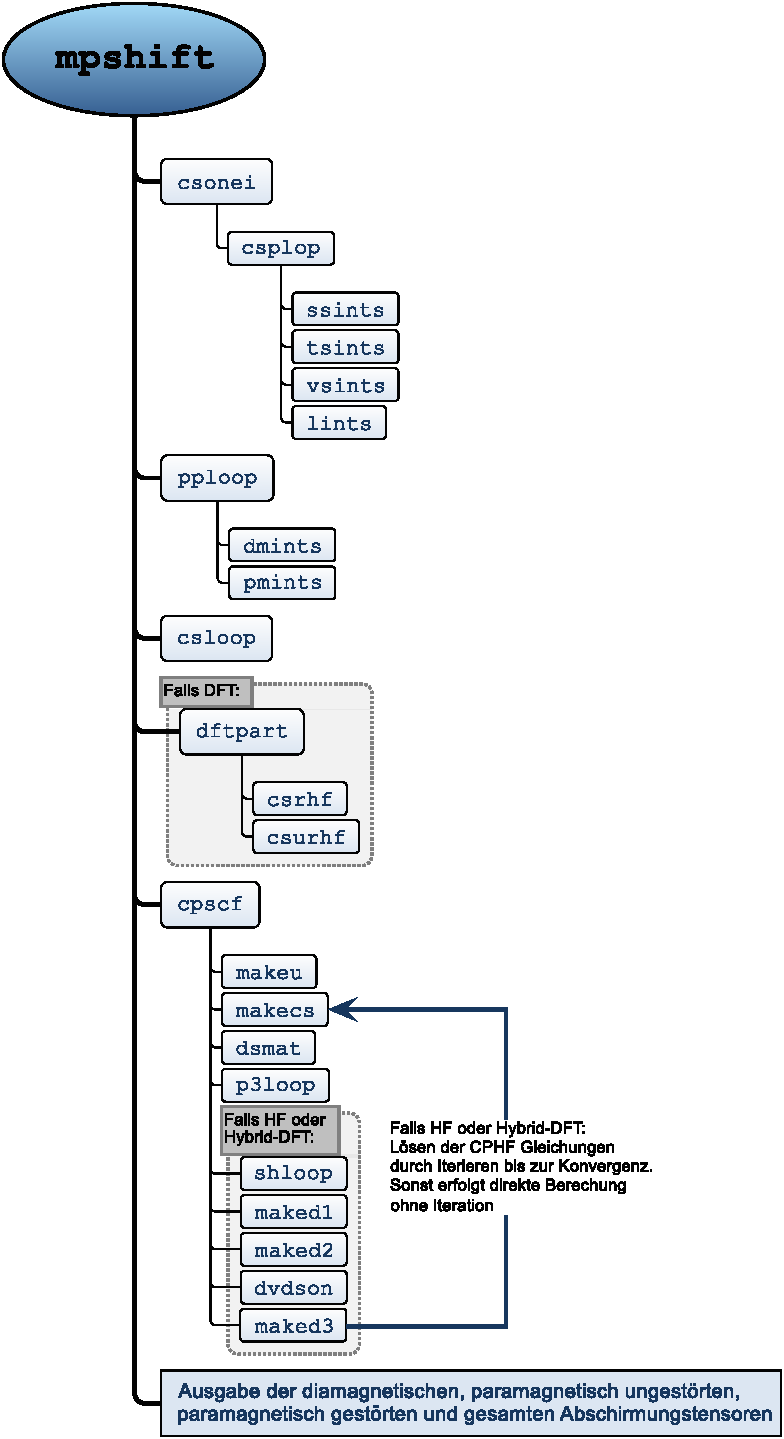
\includegraphics[width=0.75\textwidth]{programmstruktur_alt}
\captionsetup{figurewithin = chapter}
\captionsetup{font=small, labelfont=bf}\caption[Grundlegende Programmstruktur]{Schematische Darstellung der grundlegenden Programmstruktur des Moduls \texttt{mpshift} vor den Modifikationen, die im Laufe der vorliegenden Arbeit durchgeführt werden. In der Abbildung sind nur die wichtigsten Routinen enthalten.}
\label{abb:programmstrukur_alt}
\end{figure}
